% MA211 - Lecture 05
\documentclass[pdftex, xcolor=pdftex, dvipsnames]{beamer}

\usetheme{MA211}
\usepackage{thumbpdf}
\usepackage{wasysym}
%\usepackage{ucs}
\usepackage[utf8]{inputenc}
\usepackage{pgf,pgfarrows,pgfnodes,pgfautomata,pgfheaps,pgfshade}
\usepackage{verbatim}

\usepackage{eurosym}
\usepackage{euler}

\usepackage{calc}               % Simple computations with LaTeX variables
%\usepackage[hang]{caption2}     % Improved captions

\usepackage{graphicx}           % Standard graphics package

\usepackage{amsmath, amsthm, amssymb}


\newcommand{\fquad}{\mbox{\qquad}}
\newcommand{\bull}{$\bullet$ }

\newcommand {\I} {\mathcal I}
\newcommand {\calI} {\mathcal I}
\def\disint{\displaystyle\int}

\DeclareMathOperator{\D}{d}
\newcommand{\dydx}{\frac{\D y}{\D x}}

%\definecolor{gray}{rgb}{0.69, 0.69, 0.69} \newcommand{\gray}[1]{\textcolor{gray}{#1}}
\definecolor{dogreen}{rgb}{0.33, 0.42, 0.18} \newcommand{\dogreen}[1]{\textcolor{dogreen}{#1}}
\definecolor{maroon}{rgb}{.5,0.2,0.2}\newcommand{\maroon}[1]{\textcolor{maroon}{#1}}
\definecolor{greena}{rgb}{.1,0.581,0.1}\newcommand{\greena}[1]{\textcolor{greena}{#1}}

\definecolor{blue4}{rgb}{0,0,.545}
\newcommand{\Blue}[1]{\textcolor{blue}{#1}}
\newcommand{\Red}[1]{\textcolor{red}{#1}}
\definecolor{pink}{rgb}{1.,0.75,0.8}
\definecolor{darkred}{rgb}{0.5,0.0,0.0}
\definecolor{darkgreen}{rgb}{0,0.3,0.3}
\definecolor{purple}{rgb}{0,0.3,0.3}
\definecolor{darkblue}{rgb}{0.0, 0.0, .5}
\definecolor{dpurple}{rgb}{.3,.0,.3}
\newcommand{\Green}[1]{\textcolor{darkgreen}{#1}}
\newcommand{\DRed}[1]{\textcolor{darkred}{#1}}
\newcommand{\DBlue}[1]{\textcolor{darkblue}{#1}}
\newcommand{\Purple}[1]{\textcolor{dpurple}{#1}}
\newcommand{\Emph}[1]{\textcolor{darkred}{\textbf{\it #1}}}
\newcommand{\remph}[1]{\textcolor{darkred}{\textbf{\emph{#1}}}}
\newcommand{\bemph}[1]{\textcolor{darkblue}{\textbf{\emph{#1}}}}
\newcommand{\gemph}[1]{\textcolor{darkgreen}{\textbf{\emph{#1}}}}
\newcommand{\Bf}[1]{\textcolor{darkblue}{\textbf{#1}}}
\newcommand{\Gf}[1]{\textcolor{darkgreen}{\textbf{#1}}}
\newcommand{\Rf}[1]{\textcolor{red}{\textbf{#1}}}
\newcommand{\Rmf}[1]{\textcolor{red}{\mathbf{#1}}}

\newcommand{\Conj}[1]{\overline{#1}}

\newcommand{\code}[1]{\textcolor{darkblue}{\texttt{\textbf{#1}}}}
\newcommand{\icode}[1]{{\blue\texttt{\textbf{\emph{#1}}}}}
\newcommand{\gcode}[1]{{\Green{\texttt{\textbf{\emph{#1}}}}}}
\newcommand{\out}[1]{\texttt{\emph{\textbf{\Green{#1}}}}}





\newenvironment{vminipage}%
{\begin{Sbox}\begin{minipage}\begin{small}\begin{verbatim}}%
{\end{verbatim}\end{small}\end{minipage}\end{Sbox}\fbox{\TheSbox}}

\newenvironment{nminipage}%
{\begin{Sbox}\begin{minipage}}%
{\end{minipage}\end{Sbox}\fbox{\TheSbox}}


\let\Arg\relax\DeclareMathOperator{\Arg}{\mathtt{Arg}}
\let\Arg\relax\DeclareMathOperator{\e}{\mathtt{e}}

\newcommand {\AND} {\wedge}
\newcommand {\OR} {\vee}
\newcommand {\NOT} {\neg}
\newcommand {\IMPLIES} {\rightarrow}
%\newcommand {\IFF} {\leftrightarrow}
\renewcommand {\iff} {\Leftrightarrow}
\newcommand {\NAND} {\uparrow}
\newcommand {\NOR} {\downarrow}
\newcommand {\XOR} {\otimes}

\newenvironment{citemize}% Colour items
{\begin{description}}%
{\end{description}}

\newcommand {\maroonitem}{\item[\maroon{$\bullet$}]}

\newcommand {\gitem} {\item {\includegraphics[width=.4cm,angle=-10]{img/green-bullet-on-white.ps}}}
\newcommand {\ritem} {\item {\includegraphics[width=.4cm,angle=-10]{img/red-bullet-on-white.ps}}}
\newcommand {\yitem} {\item {\includegraphics[width=.4cm,angle=-10]{img/yellow-bullet-on-white.ps}}}
\newcommand {\bitem} {\item {\includegraphics[width=.4cm,angle=-10]{img/blue-bullet-on-white.ps}}}

\newcommand {\greenitem} {\item {\includegraphics[width=.4cm,angle=-10]{img/green-bullet-on-white.ps}}}
\newcommand {\reditem} {\item {\includegraphics[width=.4cm,angle=-10]{img/red-bullet-on-white.ps}}}
\newcommand {\yellowitem} {\item {\includegraphics[width=.4cm,angle=-10]{img/yellow-bullet-on-white.ps}}}
\newcommand {\blueitem} {\item {\includegraphics[width=.4cm,angle=-10]{img/blue-bullet-on-white.ps}}}

\newcommand {\eq}[1]%
  {$\DBlue{#1}$}
\newcommand {\eqd}[1]%
  {$\displaystyle\DBlue{#1}$}
%\newcommand{\eq}[1]{\boldmath \DBlue{$#1$}}


\newcommand {\csf}{\centerslidesfalse}
\newcommand {\cst}{\centerslidestrue}

\newcommand {\vecii}[2] {   \big(\begin{smallmatrix} #1 \\ #2 \end{smallmatrix}\big)}
\newcommand{\atwo}[2]{\left(\!\!\begin{array}{c} #1 \\ #2 \end{array}\!\!\right)}


\newcommand{\C}{\mathbb{C}}
\newcommand{\Q}{\mathbb{Q}}
\newcommand{\R}{\mathbb{R}}
\newcommand{\N}{\mathbb{N}}
\newcommand{\Z}{\protect\mathbb{Z}}  % protect for index.
\newcommand {\Rs}{ \mathbb{R}}
\newcommand {\Cs}{ \mathbb{C}}
\newcommand {\Rnn}{ \mathbb{R}^{n \times n}}
\newcommand {\Rn}{ \mathbb{R}^{n}}


\newcommand{\mblock}{%
\setbeamercolor*{block title}{bg=maroon,fg=white}
\setbeamercolor*{block body}{bg=white,fg=maroon}
}%

\newcommand{\bblock}{%
\setbeamercolor*{block title}{bg=Steel,fg=white}
\setbeamercolor*{block body}{bg=Mylightgray,fg=Steel}
}%

\newcommand{\gblock}{%
\setbeamercolor*{block title}{bg=Green,fg=white}
\setbeamercolor*{block body}{bg=Mylightgray,fg=darkgreen}
}%


\newcommand{\rblock}{%
\setbeamercolor*{block title}{bg=Red,fg=white}
\setbeamercolor*{block body}{bg=white,fg=Black}
}%


\newcommand{\TakeNotes}{
\includegraphics[width=2cm]{TakeNote}}

%\newcommand{\gblock}{%
%\setbeamercolor*{block title}{bg=Green,fg=white}
%\setbeamercolor*{block body}{bg=Mylightgray,fg=Green}
%}%


\def\eps{\varepsilon}
\newcommand {\del}[2]{ {\frac{\partial #1}{\partial #2}}}
\newcommand {\x}[1]{x^{[#1]}}
\newcommand {\delx}{ {\frac{\partial}{\partial x}}}
\newcommand {\delt}{ {\frac{\partial}{\partial t}}}
\newcommand {\dely}{ {\frac{\partial}{\partial y}}}
\newcommand {\ith}{{(i)}}
\renewcommand {\vec}[1]{ {\boldsymbol{#1}}}
\newcommand {\Oh} {\mathcal O}
\newcommand {\Err} {\mathcal E}
%\newcommand {\th} {\mathrm{th}}
\DeclareMathOperator{\fl}{fl}
\DeclareMathOperator{\sign}{sign}
\DeclareMathOperator{\Cond}{Cond} 
\DeclareMathOperator{\cond}{cond}
\DeclareMathOperator{\diag}{diag} 
\DeclareMathOperator{\sym}{sym} 
\DeclareMathOperator{\Trace}{Trace}
\DeclareMathOperator{\E}{e}

\newcommand {\Rsym}{{ \mathbb{R}^{n \times n}_\mathrm{sym}}}

\parskip .25cm


\theoremstyle{definition}
\newtheorem{exercise}{Exercise}[section]
\newtheorem{method}{Method}[section]



\subtitle{MA211}
\title{Lecture 5: Calculating Derivatives}

\author{Dr Niall Madden}

\date{\Large Monday 22 September 2008}


\begin{document}


\frame{

\begin{block}{}
\begin{center}
{\large \insertsubtitle}

\vspace{.1cm}

\begin{Large}
\textbf{\inserttitle}
\end{Large}

\vspace{.15cm}

% {\footnotesize \insertauthor}

\vspace{.3cm}

{ {\insertdate}}
\end{center}
\end{block}


\vspace{-0.25cm}
\begin{center}
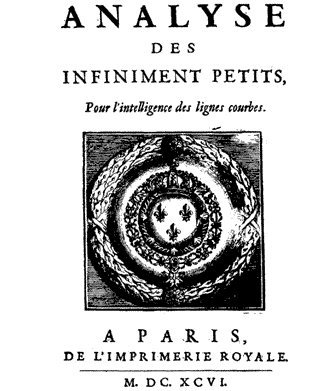
\includegraphics[height=5cm]{images/hospital1}
\end{center}
}





\frame{
\begin{center}
{\Large \Bf{Blackboard}}
\end{center}

The Blackboard site is now live. I won't be updating the pages at
\code{http://www.maths.nuigalway.ie/MA211/} 

If you are registered for MA211, you should be able to
access it. If for some reason you  can't, then send me an email.


}

\frame{

\begin{center}
{\Large \Bf{Problem Solving Sessions}}
\end{center}

\begin{block}{}
{\large \alert{Problem Solving Sessions start this week}}


\begin{itemize}

\item Tuesday, 3pm, AC202

\item Wednesday, 5pm, QA003 (Physiology lecture room)


\end{itemize}

A problem sheet will be posted to the website later today (Monday
22/09/08).

\end{block}

}

%\section{Outline}
\frame{
  \frametitle{Outline}
 \tableofcontents



}

\section{Recall... Derivatives}
\frame{
Last week we began studying the \Emph{differentiation} of functions,
and discovered that


\begin{enumerate}[<+->]
\item The formal definition of the derivative (w.r.t \eq{x}) of a
  function \eq{f} is 
\[f'(x) :=  \frac{d}{dx}f(x) := \lim_{h \rightarrow 0} \frac{ f(x+h) -
  f(x)}{h}.
\]

~

\item If \eq{f(t) = c} (a constant), then \eq{f'(t)=0}.

~

\item If \eq{f(t) = t},  then \eq{f'(t)=1}.

~

\item If \eq{f(t) = t^n},  then \eq{f'(t)=nt^{t-1}}.

\end{enumerate}

}


\frame{
More Generally:

\begin{enumerate}[<+->]
  \setcounter{enumi}{4}
\item \eq{\big(f+g\big)'(x)  = f'(x) + g'(x).}
\item \eq{\big(f-g\big)'(x)  = f'(x) - g'(x).}
\item \eq{\big(C f\big)'(x)  = Cf'(x)}, for a constant \eq{C}.

~

\item The ``\alert{Product Rule}'':  \eqd{\frac{d}{dx} ( u\cdot v)(x)  = u(x) v'(x)  +  u'(x) v(x).}

~

\item The ``\alert{Quotient Rule}''
 \eqd{\frac{d}{dx} \big(\frac{u}{v}\big)(x)  
=
\frac{v(x) u'(x)  -  u(x) v'(x)}{ \big(v(x)\big)^2}}.

~

\item These ``rules'' and the derivatives of many common functions are
  to be found on p41 and p42 of the Mathematics Tables.


\end{enumerate}


}



\section{Trigonometric function}


 
\frame{
\Bf{(See, e.g.,  Stewart \Emph{Calculus (Early Transcendentals), Section 3.2)}}


We could differentiate the trigonometrical functions $\cos$ and $\sin$
from first principles and we would find
\begin{block}{}
\[ \frac{d}{dt}\cos(t) = -\sin(t),  \]
and 
\[ \frac{d}{dt}\sin(t) = \cos(t). \]
\end{block}

\pause

The key to these proofs is that 
\[
\lim_{t \rightarrow 0} \frac{\sin(t)}{t} =0.
\]

%However, we'll see another way of doing this later...
}




\frame{

\begin{example}
Find the  derivative, with respect to \alert{$x$}  of 
\[f(t) = t+ t^2 \sin(t).\]
\end{example}

\vspace{5cm}
}


\frame{

\begin{example}
Find the  derivative, with respect to \alert{$t$}  of 
\[f(t) = t+ t^2 \sin(t).\]
\end{example}

\vspace{5cm}
}


\frame{

\begin{example}
Use the Quotient Rule to evaluate the derivative, w.r.t \eq{x} of 
\[f(x) = \frac{\sin(x)}{2x}.\]
\end{example}

\vspace{5cm}
}

\frame{

\begin{exercise}[5.1]
\begin{enumerate}[(i)]
\item Working from 1st principles, show that 
\[
\frac{d}{dx}\sin(x) = \cos(x).
\]
Hints:
\begin{itemize}
\item $\displaystyle \lim_{x \rightarrow 0} \frac{\sin(x)}{x}=1.$
\item $\sin(a+b) = \sin(a)\cos(b) + \cos(a)\sin(b)$.
\end{itemize}


\item 
Use the ``Quotient Rule'' and the fact that
\eqd{ \tan(x)= \frac{\sin(x)}{\cos(x)}}

to find the derivative of \eq{\tan(x)} with
respect to \eq{x}.
\end{enumerate}

\end{exercise}
}

\frame{

\begin{exercise}[Q5.2]
Use the product and  quotient  rules to evaluate the derivatives
  (with respect to $x$) of the following functions
\begin{enumerate}[(i)]
\item \eqd{f(x) = xe^x},
\item \eqd{f(x)=\frac{x^3}{1-x^2}}
\item $f(x)=x^2\sin(x)$
\end{enumerate}
\end{exercise}

}

\section{  Chain Rule }
\frame{
\code{(See \Emph{Calculus}, Section 3.4)}

Of all the techniques for differentiation, the most important is the
\emph{Chain Rule} for differentiating the composition of two
functions.


\begin{theorem}[The Chain Rule]
Suppose that \eq{f(x)} is defined as 
\[
f(x) = h \big( g(x)).
\]
Then
\[
\frac{df}{dx} = \frac{dh}{dg} \frac{dg}{dx}.
\]
\end{theorem}
}

\frame{

\begin{example}
Calculate the derivative of 
\[
f(x) = (x^2 -1)^3.
\]
\end{example}



\vspace{5cm}

}

\frame{

\begin{example}
Differentiate the function \eqd{f(x) = \sqrt{x^2 +1 }}
with respect to \eq{x}
\end{example}


\vspace{4cm}

}


\frame{

\begin{example}
Find the  derivative of \eqd{f(x) = e^{\sin(x)}}



\end{example}


\vspace{4cm}


}


\frame{

\begin{exercise}[Q5.3]
Use the \alert{Chain Rule} to evaluate the derivative (with respect to
\eq{x})  of each the following functions:
\begin{enumerate}[(i)]
\item \eqd{f(x) = \sin(x^2).}
\item \eqd{f(x) = \cos(k^2 + x^2).}
\item \eqd{f(x) = \frac{1}{\sqrt[3]{x^2 +x+1 }}}
\item \eqd{f(x) = \frac{x}{(x^4 +1)^3}}
\item \eqd{f(x) = xe^{-kx}}
\end{enumerate}
(Note: \eq{k} is a constant independent of \eq{x})
\end{exercise}
}


\frame{

\begin{exercise}[Q5.4]
Use the Product Rule and Chain Rule together to deduce the Quotient
Rule.
\end{exercise}
\vspace{3cm}


}



\section{l'Hospital's Rule}

\frame{

Recall again the problem of calculating limits of the form
\begin{block}{}

\[ \lim_{x \rightarrow a} \frac{f(a)}{g(a)} \]

where 
\begin{itemize}
\item \eqd{f(a) = g(a) = 0}

\item \eqd{f(a) = g(a) = \pm \infty}
\end{itemize}

Then, by \alert{l'Hospital's Rule}, 
\[  
\lim_{x \rightarrow a} \frac{f(a)}{g(a)} 
=
\lim_{x \rightarrow a} \frac{f'(a)}{g'(a)} 
\]

\end{block}
}

\frame{

\begin{example}
Evaluate the limit of the function 
\[
\frac{\log(x)}{x-1}
\]
as \eq{x} tends to \eq{1}.
\end{example}

\vspace{3cm}

}


\frame{
\begin{example}
Find \eqd{\lim_{x \rightarrow \infty} \frac{e^x}{x^2}}.
\end{example}
(Note: you can use \alert{l'Hospital's} rule repeatedly.)


\vspace{4cm}

}


\frame{
\begin{example}
Use \emph{l'Hospital's Rule} to find \eqd{\lim_{x \rightarrow 0^+} x \log(x) }
\end{example}


\vspace{4cm}

}

\frame{
\begin{exercise}[Q5.5]
Use \emph{l'Hospital's Rule} to evaluate the following limits:
\begin{enumerate}
\item \eqd{\lim_{x \rightarrow 0}\frac{\sin(x)}{x}}
\item \eqd{\lim_{x \rightarrow 0}\frac{x^2+1}{x+1}}
\item \eqd{\lim_{x \rightarrow 0}\frac{1-\cos(x)}{x^2}}
\end{enumerate}
\end{exercise}
}

\end{document}
